% t. schneider

%!TEX TS-program = xelatex
%!TEX encoding = UTF-8 Unicode

\documentclass[11pt, letterpaper]{article}
\usepackage{fontspec} 
% DOCUMENT LAYOUT
\usepackage{geometry} 
\geometry{letterpaper, textwidth=5.5in, textheight=8.5in, marginparsep=7pt, marginparwidth=.6in}

% FONTS
\defaultfontfeatures{Mapping=tex-text} % converts LaTeX specials (``quotes'' --- dashes etc.) to unicode
\setromanfont[ItalicFont={Gentium Italic}]{Gentium}


% HEADINGS
\usepackage{sectsty} 
\usepackage{float}
\usepackage{graphicx} 
\graphicspath{{../images/}}
\usepackage[normalem]{ulem} 
\sectionfont{\rmfamily\mdseries\upshape\LARGE}
\subsectionfont{\rmfamily\bfseries\upshape\Large} 
\subsubsectionfont{\rmfamily\mdseries\upshape\large} 

% PDF SETUP
% ---- FILL IN HERE THE DOC TITLE AND AUTHOR
\usepackage[dvipdfm, bookmarks, colorlinks, breaklinks, pdftitle={Goby User Manual},pdfauthor={Toby Schneider}]{hyperref}  
\hypersetup{linkcolor=blue,citecolor=blue,filecolor=black,urlcolor=blue} 
\newcommand{\xmltag}[1]{{$<$\tt #1$>$}}


% DOCUMENT

\begin{document}
\begin{figure}[H]
\begin{minipage}[b]{0.55\linewidth}
\begin{LARGE}
User Manual
\end{LARGE}
\vspace{0.5em}\\
\begin{Large}
Goby Underwater Autonomy Project
\end{Large}
\vspace{0.5em}\\
\begin{footnotesize}
T. Schneider tes@mit.edu \\
Laboratory for Autonomous Marine Sensing Systems \\
MIT / WHOI Joint Program in Oceanography \& Ocean Engineering
\end{footnotesize}
\end{minipage}
\hfill
\begin{minipage}[b]{0.3\linewidth}
\begin{flushright}

\includegraphics[width=2in]{gobysoft_logo} 
\end{flushright}
\end{minipage}
\end{figure}

\vspace{0.5em}
\rule{\textwidth}{1pt}
\vspace{0.5em}

\tableofcontents

\section{Introduction}

\subsection{What is Goby?}

The Goby Underwater Autonomy Project is an autonomy architecture\footnote{\textit{autonomy architecture}: lossly defined, a collection of software applications and libraries that facilitate communications, decision making, timing, and other utilties needed for making robots function. Another common term for this is autonomy ``middleware''} tailored for marine robotics. It can be considered a direct descendant of \href{http://www.robots.ox.ac.uk/~mobile/MOOS/wiki/pmwiki.php}{the MOOS}, with inspiration from  \href{http://code.google.com/p/lcm/}{LCM}. The motivation for Goby was the desire to seamlessly integrate \href{http://gobysoft.com/doc/acomms.html}{acoustic networking} (and other low bandwidth channels found in marine robotics) into the autonomy middleware.

Goby allows you to
\begin{itemize}
\item create custom applications\footnote{\textit{application}: a collection of code that compiles to a single exectuable unit on your operating system. synonymously (and more precise): processes or binaries} (hereafter Goby applications) that communicate with other Goby applications in a publish/subscribe\footnote{\textit{publish/subscribe}: a method of communication between processes that is roughly analogous to authors and customers of a newspaper or newsletter. Certain people (applications) publish stories (data) that other people (applications) subscribe for and read in the newsletter. Typically applications perform both tasks, subscribing for some data and publishing others. See also \url{http://en.wikipedia.org/wiki/Publish/subscribe}} manner using custom designed message objects provided by \href{http://code.google.com/apis/protocolbuffers/}{Google Protocol Buffers} project. This message passing is mediated by an application called the Goby Daemon (\texttt{gobyd})\footnote{\textit{daemon}: an application on a Linux/UNIX machine that runs continuously in the background. the \texttt{gobyd} is a server and the Goby applications are clients.}.
\item log message data using a choice of SQL\footnote{\textit{SQL}: Structured Query Language, a language (in the sense of a programming language) that allows querying or accessing data from a database. For example, if I wanted to know the best baseball players in history and I had a database of players' stats, I could write in SQL the following query that would provide the data I need: \texttt{"SELECT * FROM baseball\_players WHERE batting\_average > 0.300 ORDER BY batting\_average DESC"}} backends (\href{http://www.sqlite.org/}{SQLite3} or \href{http://www.postgresql.org/}{PostgreSQL}), allowing a choice between simplicity and power. This SQL logger is seamlessly integrated with the Google Protocol Buffers messaging. SQL provides a well-known and standards compliant way to easily access data at runtime and during post-processing.
\item log debugging output in a flexible manner to either the terminal window or a file or both, with fine-grained control over the verbosity.
\item robustly configure your Goby applications both using a text configuration file and/or command line options by writing a configuration schema in Google Protocol Buffers. Gone are the days of manual command line and configuration file parsing and validity checking. Only fields allowed in the schema are accepted by the parser, greatly reducing syntax errors in the configuration files.
\end{itemize}

\subsection{Structure of this Manual}
This manual is designed to start slow with introductory features and then ramp up to more powerful features for advanced users. Please read as far as you wish and then as soon as possible get your feet wet. In fact, you may want to go \href{http://gobysoft.com/doc}{download and install} Goby now before reading further. If you have problems, please glance at the Goby project answers (\url{https://answers.launchpad.net/goby}) or sign up for (\url{http://mailman.mit.edu/mailman/listinfo/goby}) and email the listserver \href{mailto:goby@mit.edu}{goby@mit.edu}.

\subsection{How to get help}
The Goby community is here to support you. This is an open source project so we have limited time and resources, but you will find that many are willing to contribute their help, with the hope that you will do the same as you gain experience in this area. Please consult these resources and people, probably in this order of preference:

\begin{enumerate}
\item This user manual % TODO(tes) put in link this manual
\item Questions and Answers on Launchpad: \url{https://answers.launchpad.net/goby}.
\item The developers' documentation: \url{http://gobysoft.com/doc}.
\item Email the listserver \href{mailto:goby@mit.edu}{goby@mit.edu}. Please sign up first: \url{http://mailman.mit.edu/mailman/listinfo/goby}.
\item Email the lead developer (T. Schneider): \href{mailto:tes@mit.edu}{tes@mit.edu}.
\end{enumerate}

\section{The Hello World example}

Goby is currently written entirely in C++. We hope to support more languages in the future, but we feel that C++ is a good blend of elegance, speed, and power. While the core of Goby is based on a number of advanced C++ techniques, you only need a small amount of C++ knowledge to get started writing your own Goby application. If you are new to programming and C++, we recommend Prata's \href{http://www.amazon.com/Primer-Plus-5th-Stephen-Prata/dp/0672326973}{C++ Primer Plus}. If you are experienced in programming but new to C++, we recommend Stroustrup's \href{http://www.amazon.com/C-Programming-Language-Special/dp/0201700735}{The C++ Programming Language}. The website \url{www.cplusplus.com} is an excellent online reference.

This complete example is located in \href{http://bazaar.launchpad.net/~goby-dev/goby/trunk/files/head:/src/core/examples/ex1_hello_world}{goby/src/core/examples/ex1\_hello\_world} for your reference. It's probably a good idea to \href{http://gobysoft.com/doc}{download and install} Goby now so you can try this out for yourself.

This example involves passing a single type of message (class HelloWorldMsg) from one Goby application (\texttt{hello\_world1\_g}\footnote{you can name your applications whatever you want, but we like appending ``\_g'' to the end to indicate that this is a Goby application.}) to another (\texttt{hello\_world2\_g}). Since Goby has a star topology\footnote{\textit{star topology}: all communications pass through \texttt{gobyd} and not directly from any Goby application to another}, \texttt{gobyd} will mediate this transaction.

For this example we will write two Goby applications and one Google Protocol Buffers (protobuf) message. See Fig. \ref{fig:hellow_world_structure} for the software structure of this example.

\begin{figure}
\centering
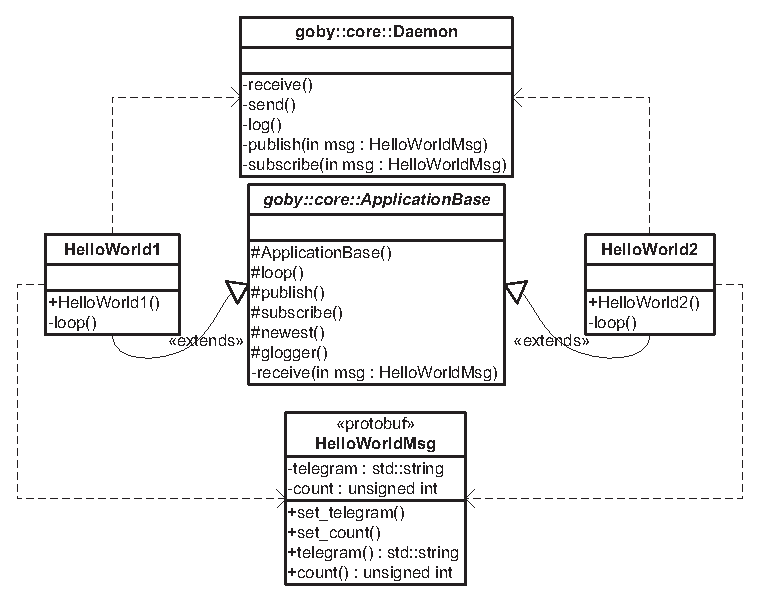
\includegraphics[scale=0.9]{hello_world_structure}
\caption{Structure diagram of the Hello World example showing the classes and dependencies. \texttt{HelloWorld1} and \texttt{HelloWorld2} are both Goby applications and thus are classes derived (solid arrows) from \texttt{goby::core::ApplicationBase}. Both of them (dashed arrows) depend on the Protocol Buffers message \texttt{HelloWorldMsg} because they use it to communicate. They also both depend on \texttt{goby::core::Daemon} (\texttt{gobyd}) for passing this message. See Fig. \ref{fig:hellow_world_sequence} for the sequence of sending a message in this example.}
\label{fig:hellow_world_structure}
\end{figure}

\subsection{Meeting goby::core::ApplicationBase}

\texttt{goby::core::ApplicationBase} is the building block (base class\footnote{also called a superclass or parent class}) upon which we will make our Goby applications (which will be derived classes \footnote{also known as subclass or child class} of ApplicationBase). \texttt{ApplicationBase} provides us with a number of tools; the main ones are:

\begin{itemize}
\item a constructor \textit{ApplicationBase()} that reads the command line and configuration (we will learn about this later) and connects to the Goby Daemon (\texttt{gobyd}) for us.
\item a virtual method \textit{loop()} that is called at a regular frequency which is 10 Hertz by default. We will learn how to change the frequency at which \textit{loop()} is called later. 
\item a method \textit{subscribe()} which tells \texttt{gobyd} that we wish to receive all messages of this type.
\item a method \textit{newest()} which returns the newest (latest received) message of a given type that we have previously called \textit{subscribe()} for. We will learn how to filter the subscriptions later.
\item a method \textit{publish()} allowing us to publish messages to \texttt{gobyd} and thereby to any subscribers of that type.
\item a method \textit{glogger()} which acts just like std::cout\footnote{\textit{glogger()} accesses an instantiation of goby::util::FlexOstream, a derived class of std::ostream. std::cout is also a derived class of std::ostream.} and lets us write to the debug (terminal window / text file) \textit{g}oby \textit{logger}.
\end{itemize}


\begin{figure}
\centering
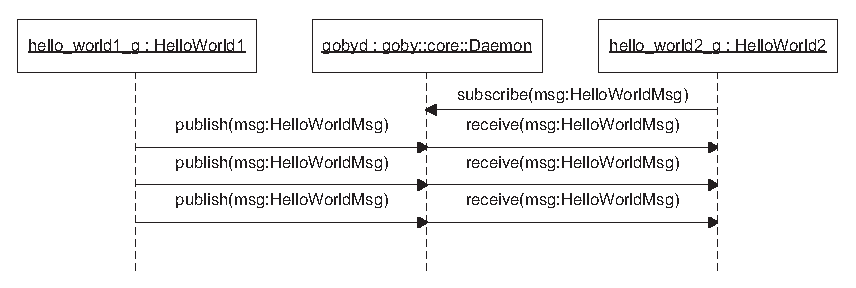
\includegraphics[scale=0.9]{hello_world_sequence}
\caption{Sequence diagram of the Hello World example. \texttt{HelloWorld2} subscribes for all messages of type \texttt{HelloWorldMsg} after which \texttt{HelloWorld1} publishes repeatedly a \texttt{HelloWorldMsg} that is processed and sent by \texttt{gobyd} to all subscribers (in this case just \texttt{HelloWorld2}).}
\label{fig:hellow_world_sequence}
\end{figure}


\subsection{Creating a simple Google Protocol Buffers Message: HelloWorldMsg}\label{sec:proto_ex}

Google Protocol Buffers\footnote{The Protocol Buffers project documented here: \url{http://code.google.com/apis/protocolbuffers/docs/overview.html}} (or protobuf for short) allows us to create custom objects for holding and transmitting data in a structured fashion. Transmitting data typically is done in a long string of bytes. However, humans do not view the world as a string of bytes. We think and communicate using tangible and intangible objects. For example, a baseball might be described by its diameter, color, weight, and materials. Goby (using protobuf objects) allows messages to be formed using this more natural representation.

The protobuf language is simple with a syntax similar to that of C. Protocol Buffers messages are written in .proto files and passed to the protobuf compiler (\texttt{protoc}) which generates C++ code to pass to the C++ compiler (\texttt{gcc} on Linux). Protobuf messages can contain a number of basic types (or vectors of these types) as well as nested messages. Fields are labeled as required, optional or repeated (essentially a vector). Required fields must be filled in; clearly, optional fields can be omitted. This might be a good time to read the \href{http://code.google.com/apis/protocolbuffers/docs/cpptutorial.html}{Protocol Buffers tutorial} to get a feel for the language and usage.

As you become familiar with using Protocol Buffers, the \href{http://code.google.com/apis/protocolbuffers/docs/proto.html}{language reference} will help you in creating .proto files and the \href{http://code.google.com/apis/protocolbuffers/docs/reference/cpp-generated.html}{generated code reference} will assist you in accessing the C++ classes created by the .proto files when passed through \texttt{protoc}.

For this example, we wish to send ``hello world'' (of course) so we need a string to hold our message that we will call `telegram'. Furthermore, we want to keep track of how many times we've said ``hello'' so we'll add an unsigned integer called `count'. The resulting \href{http://bazaar.launchpad.net/~goby-dev/goby/trunk/annotate/head:/src/core/examples/ex1_hello_world/hello_world.proto}{.proto file} should now be clear:
\begin{verbatim}
// protocol buffers language (similar to C)
message HelloWorldMsg
{
  required string telegram = 1;
  required uint32 count = 2;
}
\end{verbatim}
We chose ``required'' to prefix both fields because we feel that a valid \texttt{HelloWorldMsg} must contain both a ``telegram'' and a ``count.'' \texttt{uint32} is an unsigned (non-negative) 32 bit integer. The numbers following the ``='' sign are unique identifiers for each field. These numbers can be chosen however one likes as long as they are unique within a given protobuf message. Ascending numbers in the order fields are declared in the file is a reasonable choice.

This .proto file is ``compiled'' into a class with the same name as the message (\texttt{HelloWorldMsg}). This class is accessed by including a header file with the same name as the .proto file, but with ``.proto'' replaced with ``.pb.h''. Furthermore, we can set the contents of this class using calls (``mutators'' or ``setters'') that are the same as the field name (i.e. ``telegram'' or ''count'') prepended with ``set\_'':
\begin{verbatim}
// C++ 
#include "hello_world.pb.h"

// create and populate a ``HelloWorldMsg'' called `msg'
HelloWorldMsg msg;
msg.set_telegram("hello world");
msg.set_count(3);
\end{verbatim}

and access them using these methods (``accessors'' or ``getters'') that have the same function name as the field name:

\begin{verbatim}
// C++ 
// print information about `msg' to the screen
std::cout << msg.telegram() << ": " << msg.count() << std::endl;
\end{verbatim}


\subsection{Learning how to \textit{publish}: HelloWorld1}

To create a Goby application, one needs to

\begin{itemize}
\item create a derived class of \texttt{goby::core::ApplicationBase}. This is created by the following declaration:
\begin{verbatim}
class HelloWorld1 : public goby::core::ApplicationBase {};
\end{verbatim}
We also must include the goby core header:
\begin{verbatim}
#include "goby/core/core.h"
\end{verbatim}
\item run the application using the \textit{goby::run()} function. Because goby::core::ApplicationBase reads our configuration (including command line options) for us, we also pass argv and argc to \textit{run()}:
\begin{verbatim}
int main(int argc, char* argv[])
{   
    return goby::run<HelloWorld1>(argc, argv);
}
\end{verbatim}
\end{itemize}
That is all one needs to create a valid working Goby application. All together the ``bare-bones'' Goby application looks like:

\begin{verbatim}
#include "goby/core/core.h"

class HelloWorld1 : public goby::core::ApplicationBase {};

int main(int argc, char* argv[])
{   
    return goby::run<HelloWorld1>(argc, argv);
}
\end{verbatim}

However, we would like our application to do a little bit more.

ApplicationBase provides a \href{http://www.cplusplus.com/doc/tutorial/polymorphism/}{virtual method} called \textit{loop()} that is called on some regular interval (it is the \textit{synchronous event} in Goby), by default 10 Hertz. By overloading \textit{loop()} in our derived class \texttt{HelloWorld1}, we can do any kind of synchronous work that needs to be done without tying up the CPU all the time\footnote{in between calls to \textit{loop()}, ApplicationBase handles incoming subscribed messages}. In this example, we will create a simple message (of type HelloWorldMsg which we previously designed in section \ref{sec:proto_ex}) and publish it to \texttt{gobyd} and thus all subscribers (we create a subscriber in section \ref{sec:sub_ex}). 

Let's walk through each line of our \textit{loop()} method:

\begin{verbatim}
1 void loop()
2 {
3    static int i = 0;
4    HelloWorldMsg msg;
5    msg.set_telegram("hello world!");
6    msg.set_count(++i);
7    glogger() << "sending: " << msg << std::endl;
8    publish(msg);
9 }
\end{verbatim}

Line 1: \textit{loop()} takes no arguments and returns nothing (void). We declare (line 3) a static integer\footnote{static in this context means that the variable will keep its value across calls to the function \textit{loop()}.} to keep track of how many times we have looped and thus print an increasing integer value. Then we create a HelloWorldMsg called msg (line 4) and set the values of its fields (lines 5 and 6). We then publish a human debugging log message using \textit{glogger()} (just like std::cout or other std::ostreams), which will be put to the terminal window in verbose mode\footnote{goby provides operator<< for google::protobuf::Message objects as a wrapper for google::protobuf::Message::DebugString()}. Finally, we publish our message (line 8).

\subsection{Learning how to \textit{subscribe}: HelloWorld2} \label{sec:sub_ex}

Now that our hello\_world1\_g application is publishing a message, we would like to create an application that subscribes for it. To subscribe for a message, we typically provide two things:
\begin{itemize}
\item The type of the message we want to subscribe for (e.g. HelloWorldMsg).
\item A method or function that should be called when we receive that type (a callback).
\end{itemize}

Subscriptions typically take place in the constructor (here, HelloWorld2::HelloWorld2()), but can happen at any time as needed (within \textit{loop()}, for example). You subscribe for a type once, and then you will continue to receive all other applications' publishes to that type.

We subscribe for a type using a call to \textit{subscribe()} that looks like this:
\begin{verbatim}
subscribe<HelloWorldMsg>(&HelloWorld2::receive_msg, this);
\end{verbatim}

While a bit complicated at first, this call should make sense shortly. It reads ``\textit{subscribe} for all messages of type \textit{HelloWorldMsg} and when you receive one, call the method \textit{HelloWorld2::receive\_msg} which is a member of \textit{this} class (HelloWorld2).''\footnote{You can call a member function (method) of another class by passing the pointer to the desired class instantiation instead of \textit{this}. Alternatively, you can call a non-class function by just giving its pointer, e.g. subscribe(\&receive\_msg).}. The method provided as a callback (here \textit{receive\_msg()}) must have the signature
\begin{verbatim}
void func(const ProtoBufMessage&); 
\end{verbatim}
where ProtoBufMessage is the type subscribed for (here, HelloWorldMsg). \textit{receive\_msg()} has that signature
\begin{verbatim}
void HelloWorld2::receive_msg(const HelloWorldMsg& msg);
\end{verbatim}
and thus is a valid callback for this subscription. \textit{receive\_msg()} will be called immediately (an \textit{asynchronous} event) upon receipt of a message of type HelloWorldMsg unless
\begin{itemize}
\item \textit{loop()} is in the process of being called or
\item another message callback is in the process of being called.
\end{itemize}
In these cases, \textit{receive\_msg()} is called as soon as the blocking method returns. Inside of \textit{receive\_msg()} we simply post the message to the debug log:

\begin{verbatim}
void receive_msg(const HelloWorldMsg& msg)
{
   glogger() << "received: " << msg << std::endl;
}
\end{verbatim}

\subsection{Compiling our applications using CMake}

\href{http://www.cmake.org/}{CMake}, while still lacking in documentation, is probably the easiest way to build software these days, especially for cross platform support. I will briefly walk through building a Goby application using CMake within the larger Goby project configuration. If you look at the \texttt{CMakeLists.txt} file in \href{http://bazaar.launchpad.net/~goby-dev/goby/trunk/annotate/head:/src/core/examples/ex1_hello_world/CMakeLists.txt}{goby/src/core/examples/ex\_hello\_world/CMakeLists.txt}, you can see the steps needed to add our new applications to the project:

\begin{verbatim}
1 protobuf_generate_cpp(PROTO_SRCS PROTO_HDRS hello_world.proto)
2 add_executable(hello_world1_g hello_world1.cpp ${PROTO_SRCS} ${PROTO_HDRS})
3 target_link_libraries(hello_world1_g goby_core)
\end{verbatim}

Line 1 tells CMake to add ``hello\_world.proto'' to the files needed to be pre-compiled by the Google Protocol Buffers compiler \texttt{protoc}. protobuf\_generate\_cpp is provided by the CMake module \href{http://bazaar.launchpad.net/~goby-dev/goby/trunk/annotate/head:/cmake_modules/FindProtobufGoby.cmake}{goby/cmake\_modules/FindProtobufGoby.cmake}. Line 2 adds our application \texttt{hello\_world1\_g} to the list to be compiled by the C++ compiler, using the sources \texttt{hello\_world1.cpp} and the generated Protocol Buffers code. We append ``\_g'' as a convention to quickly recognize Goby applications. Line 3 links our application against the goby\_core library, which provides goby::core::ApplicationBase, our base class.

Adding \texttt{hello\_world2\_g} is directly analogous.

\subsection{Trying it all out: running from the command line}

Now, assuming you've \href{http://gobysoft.com/doc}{gone and compiled} everything, we can run the example.

You'll need three terminal windows, one for \texttt{gobyd}, and one for each of our ``hello world'' applications. You need to start \texttt{gobyd} first
\begin{verbatim}
> gobyd -p hello_auv
\end{verbatim}
I've gone ahead and named this platform ``hello\_auv''. The platform name is a unique identifier for both intra- and inter-vehicle communications in Goby. Now we can launch our two applications (order doesn't matter), with the added ``-v'' flag to indicate we want verbose terminal output:

\begin{verbatim}
> hello_world1_g -p hello_auv -v
> hello_world2_g -p hello_auv -v
\end{verbatim}

You should see \texttt{hello\_world1\_g} passing messages to \texttt{hello\_world2\_g} every 1/10th second.

\section{The GPS Driver example}

Marine robots need to know where they are. The simplest way now is to use a GPS receiver. While this works only when the robot is on the surface of the ocean, it is one of the most accurate forms of positioning available and thus used as a starting point for undersea dead reckoning using Doppler Velocity Loggers (DVLs) or Inertial Measurement Units (IMUs). Therefore, reading a GPS receiver's output into a usable form for decision making is a useful and necessary ability for our marine robot. This example shows how we might do this using Goby.

Typically we might also need to know the depth of our vehicle. This is often determined by measuring the ambient pressure. In this example, we will simulate the scalar depth reading of such a pressure sensor.

Finally, it is often useful to have an aggregate of the vehicle's status that includes a snapshot of the vehicle's location, orientation, speed, heading, and perhaps other factors such as battery life and health. For this example, we call such a message a ``NodeReport'' and provide an application ``node\_reporter\_g'' that compiles the reports from the GPS and the depth sensor into a single message. To extend this example, we could add data from other sources, such as an inertial measurement unit (IMU) or Doppler Velocity Logger (DVL).

As the first example, the files for this example are located in \href{http://bazaar.launchpad.net/~goby-dev/goby/trunk/files/head:/src/core/examples/ex2_gps_driver}{goby/src/core/examples/ex2\_gps\_driver} for your reference. 

\subsection{Reading configuration from files and command line: DepthSimulator}

``DepthSimulator'' is reads a starting depth value from a configuration file and reports that value as the current depth, perturbed slightly by a random value. It's a primitive constant depth simulator, but allows us to illustrate another feature of Goby, the configuration file reader.

Goby reads configuration text files and the command line also using Google Protocol Buffers. The Goby application author provides a .proto file containing a protobuf message that defines the valid configuration for the given application. Then the application instantiates a copy of this configuration message and passes it to the \texttt{goby::core::ApplicationBase} constructor with reads the configuration text file and/or command line options. If the configuration text file and/or command line options properly populate the provided proper configuration protobuf message, the message is returned to the derived class (the Goby application). Otherwise, execution of the application ends with a useful error message for the user explaining the errors involved with the passed configuration. 

Thus, for the ``DepthSimulator'' we define a protobuf message called DepthSimulatorConfig (in \href{http://bazaar.launchpad.net/~goby-dev/goby/trunk/annotate/head:/src/core/examples/ex2_gps_driver/config.proto}{goby/src/core/examples/ex2\_gps\_driver/config.proto}):

\begin{verbatim}
message DepthSimulatorConfig
{
  required AppBaseConfig base = 1;
  required double depth = 2;
}
\end{verbatim}

An embedded message of type \texttt{AppBaseConfig} is always provided for configuring parameters common for all Goby applications, such as the frequency that the virtual method \textit{loop()} is called, the name of the application to use with \texttt{gobyd} (if different from the compiled name), and the name of the platform that this application belongs on (and thus which gobyd to connect to if multiple \texttt{gobyd}s are running on a single computer). The AppBaseConfig message is defined in \href{http://bazaar.launchpad.net/~goby-dev/goby/trunk/annotate/head:/src/core/proto/app_base_config.proto}{goby/src/core/proto/app\_base\_config.proto}.

Specifically, for our DepthSimulator, we only have one other configuration parameter, a double called ``depth''. It is required, so our application will fail to run without a depth provided.

To use the Goby configuration reader, we create an instantation of our DepthSimulatorConfig
\begin{verbatim}
class DepthSimulator : public goby::core::ApplicationBase
{ 
...
    static DepthSimulatorConfig cfg_;
};
\end{verbatim}
which must either be a global object or a static member of our class so that it is instantiated before the goby::core::ApplicationBase (normal members of our DepthSimulator class would be instantiated \textit{after} ApplicationBase, which would lead to trouble when ApplicationBase tried to use the object).

Then, all we must do is pass a pointer to that object to the constructor of the base class:
\begin{verbatim}
    DepthSimulator()
        : goby::core::ApplicationBase(&cfg_)
\end{verbatim}
goby::core::ApplicationBase will take of the rest. To see what configuration values can be used in our compiled \texttt{depth\_simulator\_g}, we can run it with the -h or --help flag:
\begin{verbatim}
> depth_simulator_g --help
\end{verbatim}

which should provides output 
\begin{small}\begin{verbatim}
Allowed options:

Typically given in depth_simulator_g configuration file,
but may be specified on the command line:
  --base arg             (req)
                          platform_name: "AUV-23"  same as self.name for 
                                                   gobyd cfg (req)
                          app_name: "myapp_g"  default is compiled name - 
                                               change this to run multiple 
                                               instances (opt)
                          verbosity: QUIET  Terminal verbosity 
                                            (opt) (default)
                          loop_freq: 10  the frequency (Hz) used to run 
                                         loop() (opt) (default)
  --depth arg            (req)

Given on command line only:
  -c [ --cfg_path ] arg      path to depth_simulator_g configuration file 
                             (typically depth_simulator_g.cfg)
  -h [ --help ]              writes this help message
  -p [ --platform_name ] arg name of this platform (same as gobyd configuration
                             value `self.name`)
  -a [ --app_name ] arg      name to use when connecting to gobyd (default: 
                             depth_simulator_g)
  -v [ --verbose ] arg       output useful information to std::cout. -v is 
                             verbosity: verbose, -vv is verbosity: debug, -vvv 
                             is verbosity: gui
\end{verbatim}\end{small}

Thus, to configure \texttt{depth\_simulator\_g} I could create a text file (let's say depth\_simulator.cfg) with values like
\begin{verbatim}
# depth_simulator.cfg
base
{
    platform_name: "AUV-1"
    loop_freq: 1
}

depth: 10.4
\end{verbatim}

Then, when we run \texttt{depth\_simulator\_g} we pass the path to the configuration file as the first command line option:
\begin{verbatim}
> depth_simulator_g depth_simulator.cfg 
\end{verbatim}

If we didn't want to use a configuration file, we could pass the same contents of the depth\_simulator.cfg file given above on the command line instead:
\begin{verbatim}
> depth_simulator_g --base 'platform_name: "AUV-1" loop_freq: 1' --depth 10.4
\end{verbatim}

If the same configuration values are provided in both the configuration file and on the command line, they are merged for ``repeat'' fields. For ``required'' or ``optional'' fields, the command line value overwrites the configuration file value. 

Thus, if we run
\begin{verbatim}
> depth_simulator_g depth_simulator.cfg --depth 20.5
\end{verbatim}
\texttt{cfg\_.depth()} is 20.5 since the command line provided value takes precedence.

Some commonly used configuration values have shortcuts for the command line. For example, the following two commands are equivalent ways to set the platform name:
\begin{verbatim}
> depth_simulator_g --base 'platform_name: "AUV-1"'
> depth_simulator_g -p "AUV-1"
\end{verbatim}

Other than reading a configuration file, all ``DepthSimulator'' does is repeatedly write a message of type DepthReading (see \href{http://bazaar.launchpad.net/~goby-dev/goby/trunk/annotate/head:/src/core/examples/ex2_gps_driver/depth_reading.proto}{goby/src/core/examples/ex2\_gps\_driver/depth\_reading.proto}) based off a random offset to the configuration value ``depth'':
\begin{verbatim}
void loop()
    {
       DepthReading reading;
       // just post the depth given in the configuration file plus a small random offset
       reading.set_depth(cfg_.depth() + (rand() % 10) / 10.0);

       glogger() << reading << std::flush;
       publish(reading);    
    }
\end{verbatim}

You will note that depth\_reading.proto contains an import command and a field of type ``Header'':
\begin{verbatim}
import "goby/core/proto/header.proto";

message DepthReading
{
  // time is in header
  required Header header = 1;
  required double depth = 2;
}
\end{verbatim}

``Header'' (defined in \href{http://bazaar.launchpad.net/~goby-dev/goby/trunk/annotate/head:/src/core/proto/header.proto}{goby/src/core/proto/header.proto}) provides commonly used fields such as time and source / destination addressing. It is highly recommended to include this in messages sent through Goby, but not required. goby::core::ApplicationBase will populate any required fields in ``Header'' not given by DepthSimulator. For example, if neither time field (unix\_time nor iso\_time) is set, goby::core::ApplicationBase will set the time based on the publish time. However either unix\_time or iso\_time should be set if the calling application has a better time stamp for the message than the publish time.

\subsection{Our first ``useful'' application: GPSDriver}

GPSDriver doesn't introduce any new features of Goby, but it attempts to be the first non-trivial application we have seen thus far. GPSDriver connects to a NMEA-0183 compatible GPS receiver over a serial port, reads all the messages and parses the GGA sentence into a useful protobuf message for posting to the database (via \texttt{gobyd}). 

\subsubsection{Configuration}
The configuration needed for GPSDriver all pertains to how the serial GPS receiver is connected and how it communicates:
\begin{verbatim}
message GPSDriverConfig
{
  required AppBaseConfig base = 1;

  required string serial_port = 2;
  optional uint32 serial_baud = 3 [default = 4800];
  optional string end_line = 4 [default = "\r\n"];
}
\end{verbatim}

Note the use of defaults when they are meaningful (the NMEA-0183 specification requires carriage return and new line as the end line so this default will likely often be precisely what our users want, saving them the effort of specifying it every time).

\subsubsection{Protobuf Messages}
GPSDriver uses two protobuf messages both defined in \\ \href{http://bazaar.launchpad.net/~goby-dev/goby/trunk/annotate/head:/src/core/examples/ex2_gps_driver/gps_nmea.proto}{goby/src/core/examples/ex2\_gps\_driver/gps\_nmea.proto}. The first (NMEASentence) is a parsed version of a generic NMEA-0183 message. The second (GPSSentenceGGA) contains a NMEASentence but also parsed fields of the GGA position message. Providing the GPSSentenceGGA gives all subscribers of this message rapid access to useful data without parsing the original NMEA string again.

\subsubsection{Body}
GPSDriver should be straightforward to understand given what we have learned to this point. It makes use of some utilities in the goby::util libraries, especially the goby::util::SerialClient used for reading the serial port. These utilities are documented along with all the other Goby classes at \url{http://gobysoft.com/doc}.

Goby makes heavy use of the Boost libraries (\url{http://www.boost.org}). While you are not required to use any of Boost when developing Goby applications, it would be worth your while becoming acquainted with them. For example, the Boost Date-Time library gives a handy object oriented way to handle dates and times that far exceeds the abilities of ctime (time.h).

\subsection{Subscribing for multiple types: NodeReporter}

NodeReporter subscribes to both the output of DepthSimulator (DepthReading) and GPSDriver (GPSSentenceGGA). Whenever either is published, a new NodeReport message is created as the aggregate of pieces of both messages. The NodeReport (defined in \\ \href{http://bazaar.launchpad.net/~goby-dev/goby/trunk/annotate/head:/src/core/xamples/ex2_gps_driver/node_report.proto}{goby/src/core/examples/ex2\_gps\_driver/node\_report.proto}) is a useful summation of the status of a given node (synonomously, platform). Because DepthReading and GPSSentenceGGA are published asynchronously, we also keep track of the delays between different parts of the NodeReport message (the *\_lag fields). 

The NodeReport provides
\begin{enumerate}
\item Name of the platform
\item Type of the platform (e.g. AUV, buoy)
\item The global position of the vehicle in geodetic coordinates (latitude, longitude, depth)
\item The local position of the vehicle in a local cartesian coordinate system (x, y, z) based off the datum defined in the configuration for \texttt{gobyd}. This is generally more useful for vehicle operators than the global fix.
\item The Euler angles of the current vehicle pose: roll, pitch, yaw (heading). 
\item The speed of the vehicle.
\end{enumerate}

In this example, we only set the first three fields given above. The others would require further sensing capability than we have in this example.

\subsection{Putting it all together}



\end{document}

